\section{Jan Stopyra's Chapter}

    \textbf{Black Russian Terrier} is a dog breed that was created in the USSR around the late 40's and early 50's. It was mostly used for military work. I own one and her name is Fiona. You can see her here(See Figure \ref{fig:dog}).
\begin{figure}[h]
    \centering
    \label{fig:dog}
    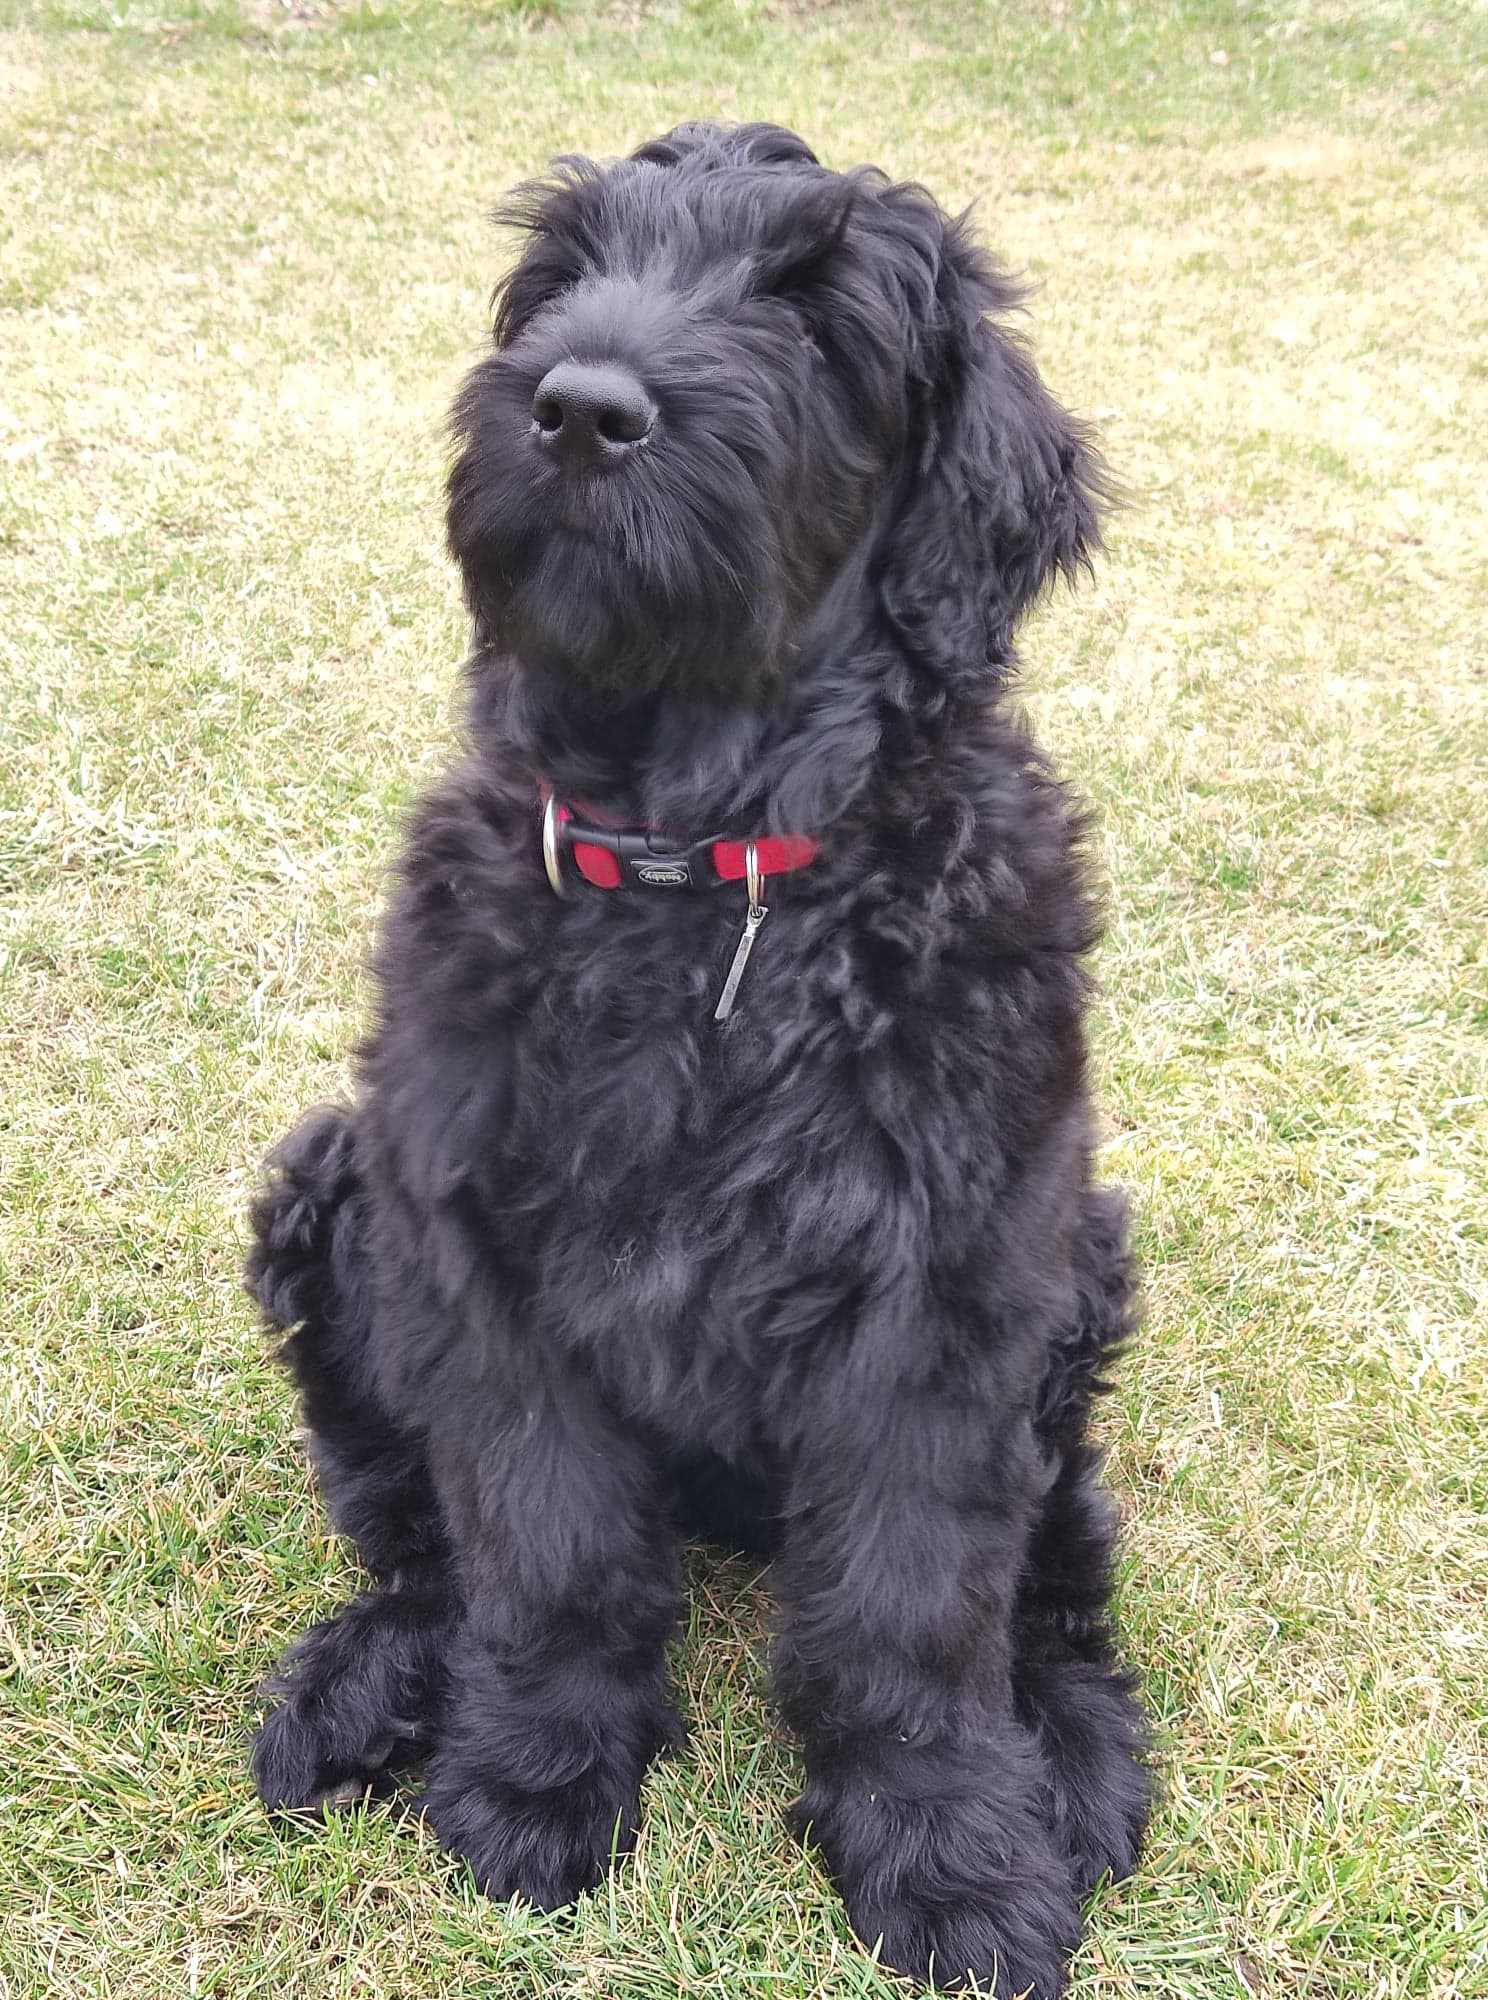
\includegraphics[width=0.3\textwidth]{Pictures/dog.jpg}
    \caption{This is a picture of the dog I have}
\end{figure}

I also like to do some \underline{math}. It's my favourite subject ever since i went to school. Here is some basic knowledge:

\begin{enumerate}

    \item Pythagoras' theorem:
        \begin{math}a^2+b^2=c^2\end{math}
    

    \item Table \ref{tab:primes} shows some interesting numbers.
    \begin{table}[htbp]
\centering
\begin{tabular}{ |c|c|c| } 
 \hline
 2 & 3 & 5 \\ \hline
 7 & 11 & 13 \\ \hline
 17 & 19 & 23 \\ \hline
\end{tabular}
 \label{tab:primes}
 \caption{This table shows the first nine prime numbers}
\end{table}
\end{enumerate}

Things to do:  
\begin{itemize}
    \item Git + GitHub
    \item LaTeX + Overleaf 
    \item Slack
\end{itemize}

